% Created 2022-08-31 Wed 11:55
% Intended LaTeX compiler: pdflatex
\documentclass[10pt]{beamer}
\usepackage[utf8]{inputenc}
\usepackage[T1]{fontenc}
\usepackage{graphicx}
\usepackage{longtable}
\usepackage{wrapfig}
\usepackage{rotating}
\usepackage[normalem]{ulem}
\usepackage{amsmath}
\usepackage{amssymb}
\usepackage{capt-of}
\usepackage{hyperref}
\usepackage{minted}
\usepackage[T1]{fontenc}
\usepackage{pmboxdraw}
\usetheme{Berkeley}
\usefonttheme{professionalfonts}
\usepackage{booktabs}
\definecolor{mycolor}{rgb}{0.54706, 0.13725, 0.26667}
\usecolortheme[named=mycolor]{structure}
\setlength{\parskip}{5pt}
\newcommand{\footnoteframe}[1]{\footnote[frame]{#1}}
\addtobeamertemplate{footnote}{}{\vspace{2ex}}
\usepackage{xcolor}
\definecolor{LightGray}{gray}{0.95}
\usepackage{fancyvrb}
\DefineVerbatimEnvironment{verbatim}{Verbatim}{fontsize=\scriptsize}
\DeclareGraphicsRule{.gif}{png}{.png}{`convert #1 `dirname #1`/`basename #1 .gif`-gif-converted-to.png}
\DeclareGraphicsExtensions{.gif}
\usepackage{animate}
\author{Jay Morgan}
\date{<TODO>}
\title{Machine Learning\\\medskip
\large Lab 1 - Linear Models}
\hypersetup{
 pdfauthor={Jay Morgan},
 pdftitle={Machine Learning},
 pdfkeywords={},
 pdfsubject={},
 pdfcreator={Emacs 28.1 (Org mode 9.5.4)}, 
 pdflang={English}}
\begin{document}

\maketitle

\section*{Introduction}
\label{sec:org62f0ee8}

\subsection*{Plan for this lab}
\label{sec:org210c2db}

\subsubsection*{Welcome}
\label{sec:org7ddf871}

Welcome to the first lab. In these lab tutorials we are going to be experimenting
with what we've learnt in the lectures. This means that we're going to implement the
algorithms and doing some Machine Learning ourselves!

\subsubsection*{Plan for the first lab}
\label{sec:orgb545ac0}

For this first lab session, we're going to need to do just a little 'admin' work
before we start implementing these algorithms.

We will need to do the following:
\begin{itemize}
\item Create an project directory.
\item Create a conda environment and install the latest version of Python.
\item Setup our IDE (integrated development environment of choice).
\end{itemize}

\subsection*{Lab setup}
\label{sec:org46b5c9b}

\subsubsection*{Creating a project directory}
\label{sec:org4eca51e}

Exactly how you want to organise your work is up to you. However, with that being
said, I would recommend the following example structure:

\begin{verbatim}
~/workspace/<project-name>/<files-&-directories>
\end{verbatim}

So, for example, in this course, we would have the following directory:
\texttt{\textasciitilde{}/workspace/machine-learning}

\subsubsection*{Using the datascience repository}
\label{sec:orgaf46b82}

\begin{figure}[htbp]
\centering
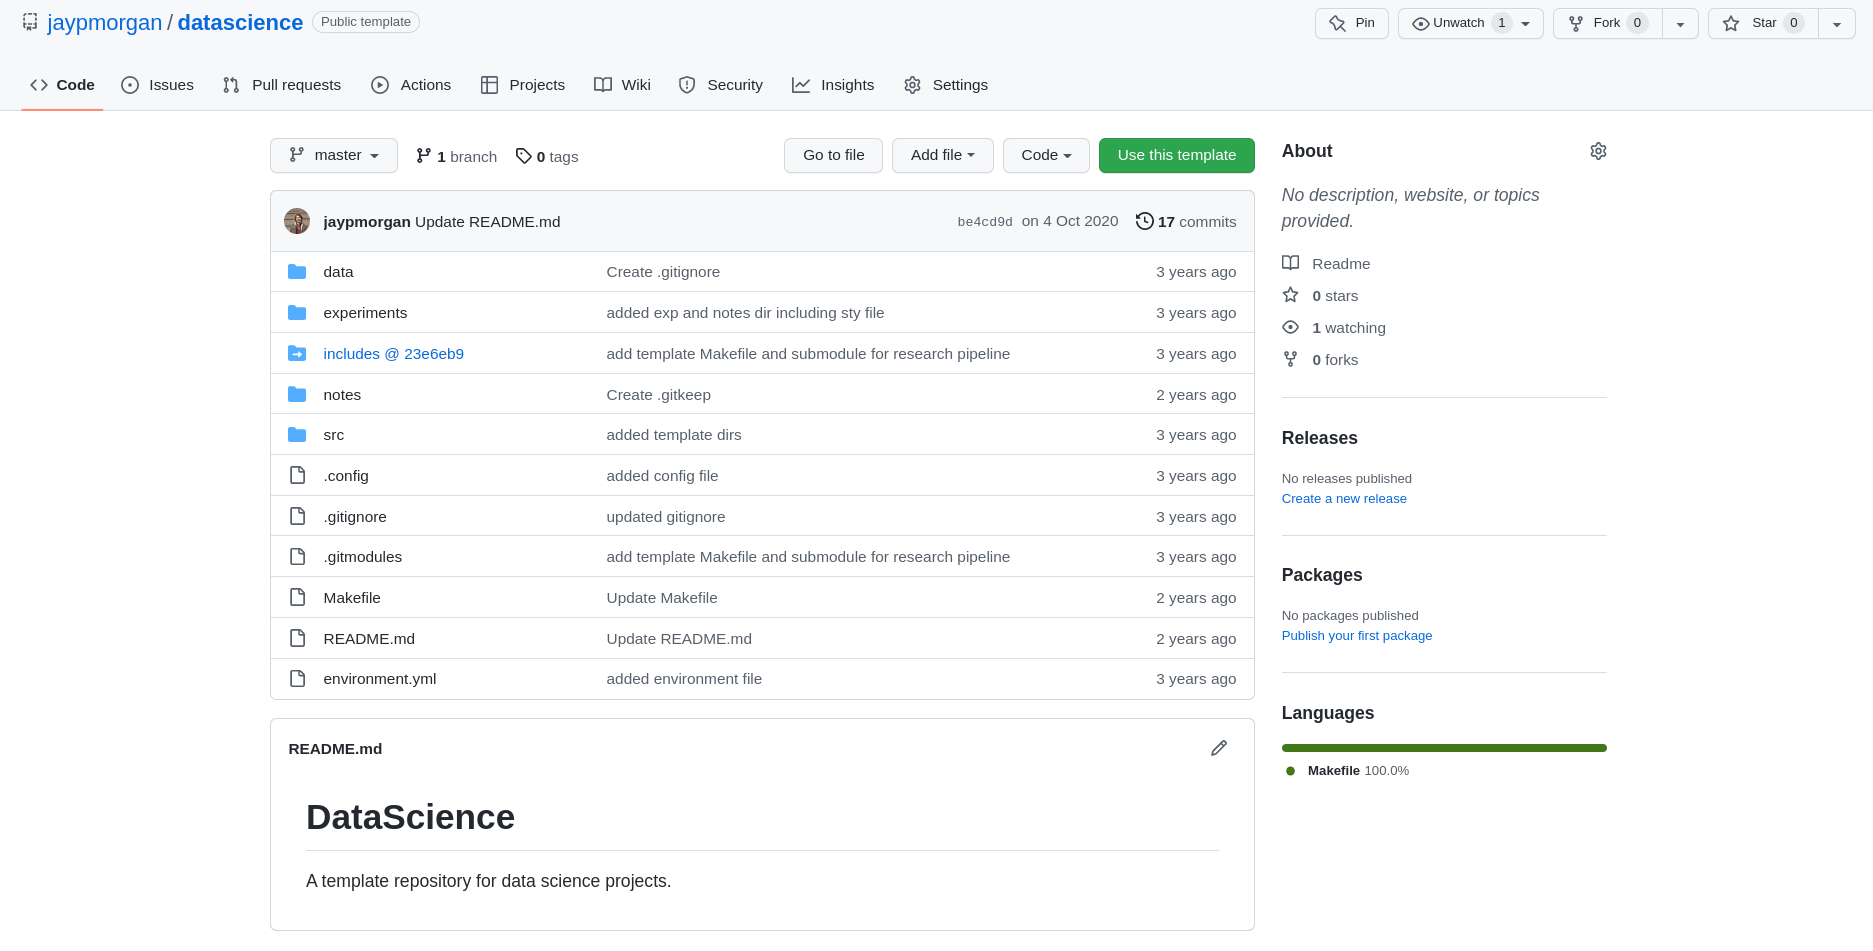
\includegraphics[width=.9\linewidth]{images/datascience-repo.png}
\caption{The datascience repository templated hosted on github (github.com/jaypmorgan/datascience)}
\end{figure} 

\begin{minted}[]{bash}
git clone git@github.com:jaypmorgan/datascience.git
\end{minted}

\subsubsection*{Layout \& intentionality behind the datascience repository}
\label{sec:org176639f}
\begin{itemize}
\item \texttt{data} -- location of all data files (preferably in their own directory such as
data/raw/<files>, data/processed/<files>, data/results/<files>). These files will
not be committed to git as they much be too large.
\item \texttt{experiments} -- location of one off files that are used for running single
experiments and scripts.
\item \texttt{notes} -- storage of notes and reports created during the lifetime of the project.
\item \texttt{src} -- here we store the library of functions/classes that are useful for the
entire project.
\item \texttt{.config} -- a configuration file
\item \texttt{Makefile} -- make routines for building the project (if we have any, we'll cover
this at a later point, alternatively you can read:
\url{https://blog.morganwastaken.com/2020-03-05/makefile}).
\item \texttt{environment.yml} -- the configuration script for conda (we'll cover this just in a
moment!).
\item \texttt{README.md} -- Markdown readme file that explains introduces the project, and perhaps
some installation and running instructions for others.
\end{itemize}

I will using this folder structure for our labs, so we'll see (by the way of example)
how we use this structure.

\subsubsection*{Creating a conda environment}
\label{sec:org91b9e38}

Conda is a command line tool to manage environments. We're going to highlight some of the most used commands. But for the full list of management, you can use the instructions at: \url{https://conda.io/projects/conda/en/latest/user-guide/tasks/manage-environments.html}

If you're creating a brand new environment, use:

\begin{verbatim}
conda create --name <name-of-env>
\end{verbatim}

This will prompt you to confirm you want to create a new environment, whereupon you
enter either a y or n. If y your new environment will be created, but start using the
environment, you will first have to activate it.

For more information, visit:
\url{https://pageperso.lis-lab.fr/jay.morgan/resources/2021-programming-level-up/lectures/week-3/lecture.html\#orga9fbc8c}


\subsubsection*{Installing jupyter notebook \& jupyter lab}
\label{sec:org6aa2fc5}

As we're going to do lots of visualisations, we're going to want some environment
where we can rapidly evolve and interrogate our data. For this, we're going to use
jupyter notebooks. However, there are many other alternatives if you're so
inclined. There is google colab (a jupyter-like environment on the cloud), org-mode
with org-babel if you like emacs, the Spyder IDE with code cells.

To install jupyter notebook use (assuming you have activated the correct environment):

\begin{minted}[]{bash}
conda install -c conda-forge jupyterlab
\end{minted}

\url{https://jupyterlab.readthedocs.io/en/stable/getting\_started/installation.html}

\subsubsection*{Setting up our IDE}
\label{sec:orgf2c8222}

While most of our exploration is going to take place inside a jupyter notebook,
we're going to use a fully fledged IDE for the heavy lifting of our Python
programming. The IDE we're going to use in these lab sessions is PyCharm.

\begin{figure}[htbp]
\centering

\includegraphics[width=.9\linewidth]{images/pycharm.png}
\caption{PyCharm IDE}
\end{figure}

\section*{Creating a linear model}
\label{sec:orgcc624c0}

\subsection*{Data}
\label{sec:org0b3b10e}

\subsubsection*{Getting the data}
\label{sec:org6f5d1e1}
\end{document}
